\documentclass{CRPITStyle}


\usepackage{harvard}
\usepackage{graphicx}
\usepackage{verbatim}


\pagestyle{empty}
\thispagestyle{empty}


\title{Lightweight Update Propagation using Atom}
\author{David W.\ Williamson \and Nigel J.\ Stanger}
\affiliation{Department of Information Science, \\
	University of Otago, \\
	PO Box 56, Dunedin, New Zealand \\
	Email:~\texttt{\{dwilliamson,nstanger\}@infoscience.otago.ac.nz}}


\begin{document}


\maketitle


\begin{abstract}
There are many situations where some form of automated update
propagation across disparate databases may be beneficial. For example, a
retailer could automatically retrieve the latest pricing data from their
suppliers' databases, and use these data to update their own internal
database. Doing so at regular intervals ensures that the retailer always
has current pricing information in their database. Electronic Data
Integration (EDI) tools that provide such features already exist but can
be expensive to implement, particularly for small to medium enterprises
(SME's). In this paper we propose a lightweight approach for propagating
updates from one database to another using the Atom XML syndication
format, thus providing a simpler, cost-effective technology for
facilitating data integration. This approach enables a target database
to regularly query one or more source databases for updates, which are
then applied to the target database (alternatively, updates could be
``pushed'' to the target from the sources). This approach can be used in
typical data integration scenarios where the data sources are updated at
irregular intervals, such as the aforementioned retailer example, or
when extracting data from multiple data sources for loading into a data
warehouse. In the paper we discuss the underlying principles and
motivation for the approach, discuss possible architectures, and
describe an early prototype implementation.
\end{abstract}
\vspace{.1in}

\noindent {\em Keywords:} update propagation, data integration, Atom,
Semantic Web, B2B


\section{Introduction}
\label{sec-intro}

The ability to integrate data from multiple heterogeneous sources is
becoming a key issue for modern businesses, yet the number of businesses
implementing data integration solutions is smaller than we might expect
\cite{Beck-R-2002-Bled,vaHe-E-1999-EDI}. This is particularly true for
small to medium enterprises (SME's), for whom the cost of implementing
an enterprise-scale data integration solution can often be prohibitive
\cite{Beck-R-2002-Bled,Guo-J-2003-DocEng,Somm-RA-2002-SIGMOD}.

In this paper, we propose a lightweight approach for propagating updates
from one database to another using the Atom XML syndication format. This
approach could provide a cost-effective alternative technology for SME's
to facilitate data integration rather than having to purchase expensive
enterprise grade systems. The underlying architecture is very flexible
and can be easily extended to support additional functionality.

We should clarify at this point that we are not proposing an approach
for processing data streams \cite{Babc-B-2002-Streams}. Such approaches
deal with processing continuous streams of real-time data, whereas our
approach provides a lightweight means to propagate discrete sets of
``conventional'' update operations from one database to another.

The remainder of this paper comprises seven sections. In
Section~\ref{sec-background} we provide some general background
information regarding data integration and the Atom syndication format,
while in Section~\ref{sec-motivation} we discuss the motivation behind
our approach. We outline the architecture underlying our approach in
Section~\ref{sec-architecture} and discuss the implementation and
testing of a proof of concept prototype in Section~\ref{sec-prototype}.
Preliminary results of the testing are presented in
Section~\ref{sec-results}, followed by possible directions for future
work in Section~\ref{sec-future-work}. The paper concludes in
Section~\ref{sec-conclusion}.


\section{Background}
\label{sec-background}

In this section, we briefly discuss the concepts and technologies that
underlie our approach. In Section~\ref{sec-data-integration} we provide
a brief overview of data integration, especially in the context of SME's
attempting to implement a data integration solution. This is followed by
a brief discussion of the development of Atom and related technologies
such as RSS and RDF.


\subsection{Data Integration}
\label{sec-data-integration}

Data integration is a term used to describe the combining of data
residing in different sources to provide the user with a unified view of
those data \cite{Bati-C-1986,Yu-C-2004-SIGMOD}. This activity is
becoming increasingly important to modern business operations as more
and more organisations rely upon applications that support staff in
undertaking informed decision making
\cite{Calv-D-1998-CoopIS,Yu-C-2004-SIGMOD}.

Data integration is a domain that has been a topic of research for some
time \cite{Beck-R-2002-Bled,Wied-G-1993-SIGMOD}; today this domain is of
no less significance with many organisations requiring the aggregation
of data from multiple and often heterogeneous sources, for a wide
variety of applications \cite{Haas-LM-1999-DEB}.
\citeasnoun{Bati-C-1986} illustrated three common scenarios for
integration environments:

\begin{enumerate}

	\item homogeneous, where all the sources of data share the same
	schema;

	\item heterogeneous, where data must be integrated from sources that
	may use different schemas or platforms (e.g., a combination of
	relational and hierarchical databases); and

	\item federated, where integration is facilitated by the use of a
	common export schema over all data sources.

\end{enumerate}

A typical example of data integration from heterogeneous sources can be
found in the arena of business-to-business (B2B) commerce, where, for
example, a manufacturer may have to interact with multiple suppliers or
temporary contractors, each of whom may use completely different data
structures and data exchange formats \cite{Ston-M-2001-SIGMOD}. With the
introduction of cheaper web-based technology, many more organisations
have been able to undertake projects to facilitate data integration, but
the costs associated with such technology can still be quite prohibitive
to the many smaller companies and organisations that comprise the
majority of most countries' economies.

Many initiatives have been put forward to try and alleviate this
situation, one of the more recent being the OASIS Universal Business
Language (UBL) standard \cite{Mead-B-2004-UBL}, which is a project to
standardise common business documentation---invoices, purchase orders,
etc.---so that it is easier for companies to establish and maintain
automated transactions with other parties. UBL has been designed to
operate with another OASIS standard, ebXML \cite{Eise-B-2001-ebXML},
which specifies a framework for facilitating e-business transactions.

XML has been widely adopted as a standard platform for exchanging data
between organisations, and many specialist standards---such as the
aforementioned ebXML---have been developed to cater to the unique needs
that certain business sectors present. In addition to XML-based language
specifications, other standards such as EDIFACT and EXPRESS have been
defined to facilitate the transmission of information from various
sources so that it may be integrated with other data.


\subsection{The Atom Syndication Format}
\label{sec-atom-overview}

In this section we provide a brief overview of the Atom syndication
format and the technologies that led to its development.


\subsubsection{RDF, RSS and the Semantic Web}
\label{sec-rdf-rss}

The World Wide Web (WWW) as it stands today mostly comprises documents
intended for humans to read, i.e., ``\ldots{}a medium of documents for
people rather than for data and information that can be processed
automatically\ldots'' \cite{Bern-T-2001-SciAm}, which provides minimal
opportunity for computers to perform additional interpretation or
processing on them \cite{Bern-T-1999-WWW,Bern-T-2001-SciAm}. In essence,
computers in use on the web today are primarily concerned with the
parsing of elementary layout information, for example headers, graphics
or text, and processing like user input forms
\cite{Bern-T-1999-W3C,Bern-T-2001-SciAm}.

There are few means by which computers can perform more powerful
processing or manipulation on web resources
\cite{Bern-T-2001-SciAm,Fens-D-2003}, most often because the additional
semantics required do not exist or are not in a form that can be
interpreted by computers \cite{Koiv-MR-2001-W3C}. The motivation for the
adoption of semantics in web documents can be made evident simply by
using a contemporary search engine to look for an ``address''. This
search may well return a plethora of results ranging from street
addresses and email addresses to public addresses made by important
individuals through the ages.

This kind of scenario is one of the reasons for the W3C's Semantic Web
project \cite{Koiv-MR-2001-W3C}. In the words of its creator, Tim
Berners-Lee, its goal is to:

\begin{quotation}
	``\ldots{}develop enabling standards and technologies designed to
	help machines understand more information on the Web so that they
	can support richer discovery, data integration, navigation, and
	automation of tasks. With Semantic Web we not only receive more
	exact results when searching for information, but also know when we
	can integrate information from different sources, know what
	information to compare, and can provide all kinds of automated
	services in different domains from future home and digital libraries
	to electronic business and health services.''
	\cite{Koiv-MR-2001-W3C}
\end{quotation}

RDF is a technology that is an integral part of the W3C Semantic Web
initiative, as the following excerpt from the W3C Semantic Web activity
statement will attest:

\begin{quotation}
	``The Resource Description Framework (RDF) is a language designed to
	support the Semantic Web, in much the same way that HTML is the
	language that helped initiate the original Web. RDF is a framework
	for supporting resource description, or metadata (data about data),
	for the Web. RDF provides common structure that can be used for
	interoperable XML data exchange.'' \cite{Powe-S-2003-RDF}
\end{quotation}

What RDF does in the context of the Semantic Web is to provide a way to
record data so that they can be interpreted easily by machines, which in
turn provides an avenue to ``\ldots{}more efficient and sophisticated
data interchange, searching, cataloguing, navigation, classification and
so on\ldots{}'' \cite{Powe-S-2003-RDF}.

Since its inception in the late 1990's, the RDF specification has
spawned several applications, RDF Site Summary (RSS) being but one
example. Versions 0.9 and 1.0 of RSS conform to the W3C's RDF
specification. It is a format intended for metadata description and
content syndication \cite{Mano-F-2004-RDF}. Originally developed by
Netscape as a means to syndicate content from multiple sources onto one
page \cite{Nott-M-2005-Atom}, RSS has been embraced by other individuals
and organisations resulting in the spawning of multiple versions.

At its most simple, the information provided in an RSS document
comprises the description of a ``channel'' (which could be on a specific
topic such as current events, sport, weather, etc.) consisting of URL
linked items. Each item comprises a title, a link to the actual content
and a brief description or abstract. In essence, RSS provides a simple
way to summarise changes to a web site in a form that is easy to access
and process.

Because of the proliferation of differing RSS standards and associated
problems with compatibility, a group of service providers, vendors and
developers have initiated the development of a separate syndication
standard named Atom. According to the Atom Publishing Format and
Protocol (Atompub) Working Group, the development of Atom is heavily
influenced by the lessons learned in the evolution of RSS.


\subsubsection{Atom}
\label{sec-atom-detail}

The Atom specification defines an XML-based document format that is
designed to describe lists of related information
\cite{Nott-M-2005-Atom}. These lists are known as ``feeds''. Feeds are
made up of multiple items, known as ``entries''; each entry can have an
extensible set of attached metadata \cite{Nott-M-2005-Atom}.
Figure~\ref{fig-atom-example} shows an example of a simple, single-entry
Atom feed document.


\begin{figure}
	\fbox{\parbox[b]{.99\linewidth}{%
		\vskip 0.5cm%
		\footnotesize%
		\verbatiminput{feed.atom}%
		\vskip 0.25cm%
	}}
	\caption{A simple, single-entry Atom feed document \protect\cite{Nott-M-2005-Atom}}
	\label{fig-atom-example}
\end{figure}


Atom as a technology comprises four key related components: a conceptual
model of a resource, a well defined syntax for this model, the actual
atom feed format itself and an editing protocol. Both the feed format
and editing protocol also make use of the aforementioned syntax.

The latest Atom specification (1.1), which at the time of writing is
still in draft form, states that the main use case that Atom is intended
to address is ``\ldots{}the syndication of Web content such as Weblogs
and news headlines to Web sites as well as directly to user agents''
\cite{Nott-M-2005-Atom}. The specification also suggests, however, that
Atom should not be limited to just web based content syndication but in
fact could be adapted for other uses or content types. The Atompub
Working Group have submitted the Atom feed format and editing protocol
to the IETF for consideration as an Internet standard.


\section{Motivation}
\label{sec-motivation}

One of the example domains of data integration is that of Electronic
Data Interchange (EDI), a concept used by companies to exchange
information such as goods procurement documentation. EDI is not new
\cite{Beck-R-2002-Bled,Medj-B-2003-VLDB}, and has been used for many
years by various organisations to reduce costs by replacing more
traditional paper based systems. It is interesting to note, however,
that in surveys regarding the extent of EDI adoption, only a fraction
of the companies that might be perceived as beneficiaries of such
technology have actually implemented or attempted to implement it
\cite{Beck-R-2002-Bled,vaHe-E-1999-EDI}. This naturally raises the
question of why this is the case. We can further refine this question by
asking why so few smaller companies (SME's) have adopted EDI or indeed
other technologies that rely on accurate automated data integration,
such as data warehousing.

Perhaps the most important reason is that of cost: to a small company
the perceived benefits of introducing the technology may not be
sufficient to justify the expense
\cite{Beck-R-2002-Bled,Guo-J-2003-DocEng,Somm-RA-2002-SIGMOD}. When a
decision has been made to implement such technology, it is often the
case that the SME in question has been forced into an investment that
is, to them, an expensive solution, perhaps due to demands imposed by
larger clients and partners, or as a response to competitors in an
attempt to maintain market position
\cite{Beck-R-2002-Bled,vaHe-E-1999-EDI}.

Attempts have been made to make EDI more cost effective by introducing
EDI on a web-based platform \cite{Beck-R-2002-Bled}, and through the
development of standards such as UBL \cite{Mead-B-2004-UBL}. While UBL
is new and has probably not had sufficient time to make a substantial
impact, the fact remains that the underlying reason these types of
technologies are still not attractive enough to SME's is cost
\cite{Beck-R-2002-Bled,Guo-J-2003-DocEng,Somm-RA-2002-SIGMOD,vaHe-E-1999-EDI}.

To summarise, data integration related technologies are often not
readily or willingly implemented by SME's because of the perceived high
costs involved, and at best are implemented only if it is deemed vitally
important to the continued survival of the organisation in the
marketplace.

Such a situation leads us to the conclusion that there is a need for
alternative, cost-effective technologies to facilitate data integration,
enabling SME's to embrace the benefits of applications that rely on data
integration, such as data warehousing, EDI networks or e-catalogues.
This identified need provides the motivation for our approach, which we
will now discuss.


\section{Update Propagation using Atom}
\label{sec-architecture}

To facilitate the adoption of data integration in SME's, we propose a
lightweight approach for propagating database updates based on Atom,
as illustrated in Figure~\ref{fig-basic}. Atom was chosen as the
underlying technology because of its XML heritage, and because the Atom
community is trying to encourage different uses beyond
the traditional application of weblog syndication
\cite{Nott-M-2005-Atom}. Although the standard has yet to be officially
ratified, it already has a large user and development community.

Figure~\ref{fig-basic} shows a basic architecture for our approach. A
feed generator queries its corresponding data source and compares the
results against a snapshot stored in a small staging database. If the
latest query results differ from the snapshot, then updates have
occurred in the data source, and a new version of the Atom feed is
generated. The latest query results replace the snapshot in the staging
database. The Atom feed is then read by a feed consumer, which
reconstructs the database updates and applies them to the target
database.


\begin{figure*}[htb]
	\fbox{\parbox[b]{.99\linewidth}{%
		\vskip 0.5cm%
		\centerline{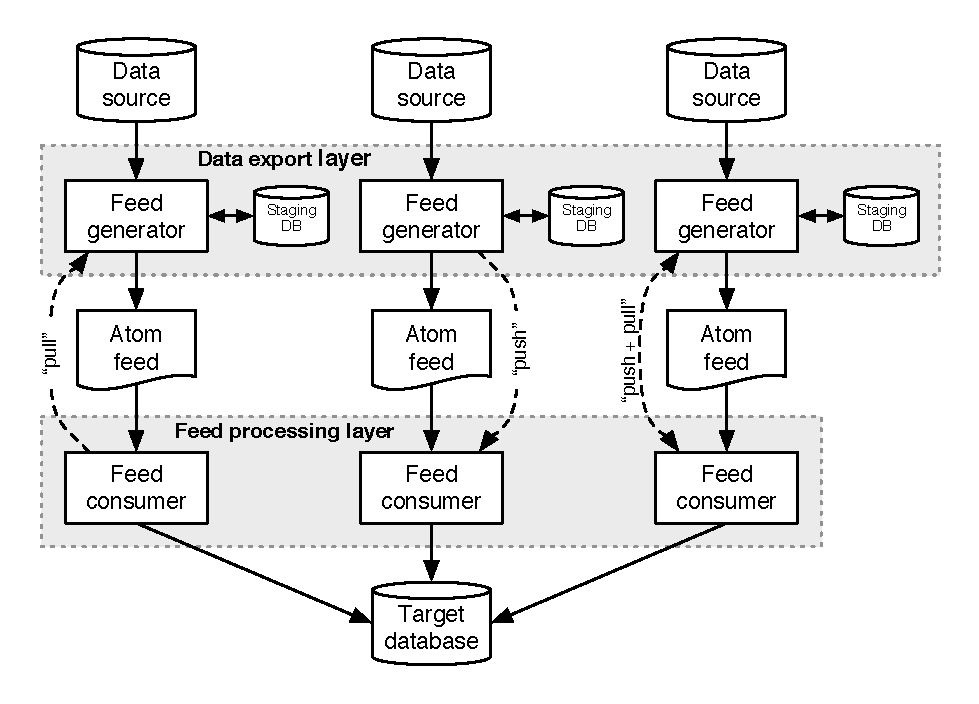
\includegraphics[scale=0.9]{Architecture_basic}}%
		\vskip 0.5cm%
	}}
	\caption{Overview of the basic architecture}
	\label{fig-basic}
\end{figure*}


In the typical use case of weblog syndication, Atom feeds are polled by
clients at regular intervals, and the client determines whether the feed
has changed by comparing the modification time of the feed (encoded in
the \verb|<updated>| element in Figure~\ref{fig-atom-example}) against
the time that the client last checked. This may not be an optimal
approach for propagating database updates, however. If a client polls
the feed less frequently than updates occur at the data source, there is
a danger of updates being lost, as the corresponding entries in the feed
may ``scroll off the end''before the client has a chance to see them.
This is particularly of our approach, where each new set of updates to a
data source results in a completely new feed being generated. A simple
polling model is therefore inappropriate.

This issue is resolved in our approach by enabling direct communication
between the feed generator and its corresponding feed consumer(s). There
are two methods of achieving this, as indicated by the ``push'' and
``pull'' annotations in Figure~\ref{fig-basic}. In the ``push'' method,
the consumption of feed information is driven primarily by changes in
the source data. When the generator detects such a change (for example,
when a record is updated), it regenerates the feed, then directly
notifies its corresponding consumers, thus ``pushing'' the updates to
the consumers. (Alternatively, the consumers could be said to be
listening for update events from the generator.)

The ``pull'' method is the converse of the push method, in that the flow
of feed information to the target schema is governed by the consumer
itself. Rather than polling a ``static'' feed file, the consumer
requests its corresponding generator to dynamically generate a custom
feed as required. In other words, the consumer ``pulls'' the updates
from the generator. This method may be more suited to a situation where
there are multiple consumers associated with one generator (this is not
shown in Figure~\ref{fig-basic}). The generator may need to maintain
separate snapshots for each of its consumers in such cases, as the
consumers might have different request frequencies.

Both methods have their place, and indeed could be combined, as shown on
the right of Figure~\ref{fig-basic}. That is, a generator could generate
a ``static'' feed at regular intervals and notify its consumers, while
also responding to requests for dynamic feeds from its consumers.

Figure~\ref{fig-basic} provides no indication as to where on the network
these different components will execute. In practice the precise
location of each component is not critical, as long as they are able to
communicate with each other. Thus, for example, the generator and
consumer could both reside on the source machine, or the generator could
reside on the source machine while the consumer resides on the target
machine, or they could reside on machines separate from both the source
and target.


\section{Prototype Implementation and Testing}
\label{sec-prototype}

We have implemented a basic proof of concept prototype using PHP 5, in
order to explore implementation issues and to do some initial
scalability testing. The prototype currently supports only the push
method and works only with the MySQL and PostgreSQL database management
systems (DBMS). PHP was chosen because of its excellent DBMS support and
because it enabled us to quickly create web-based modules that could
easily call each other by means of HTTP redirects.

In order to provide context for implementing and evaluating the
prototype, we have developed two simulated scenarios derived from actual
use cases of previous projects. Both case studies follow a similar
structure whereby data are exported as Atom feeds from the source
database(s), then read by a feed consumer before being sent to the
target database.

The first scenario simulates the integration of movie timetable data
from multiple cinema databases (the sources) into a vendor's movie
timetable database (the target). This database is used to populate an
e-catalogue allowing users to query times and locations of movies
currently screening at the cinemas who contribute data to the system.
The Atom feeds in this scenario represent flows of data from the
supplier (the participating cinemas) to the vendor (the e-catalogue
provider).

The second scenario follows on from an earlier research project at the
University of Otago to develop a kiosk-based system for the sale and
distribution of digital music (e.g., MP3 files). The database in the
kiosk is initially populated with information provided by music vendors,
and updates to the suppliers' databases (the sources) are then
propagated to the music kiosk database (the target). The Atom feeds in
this instance are used to maintain an up to date database at the kiosk,
which has the location and description of each music track for sale in
the system.

Both case studies vary in terms of complexity of design and
implementation demands, enabling us to pursue a staged development of
the core components. We first implemented the less complex movie
e-catalogue case study, then used our experiences from this to extend
the prototype to support the music kiosk case study.

Testing of essential functionality has been carried out on the movie
e-catalogue system, but the main focus for extensive testing has been on
the music kiosk retail system. Not only does the music kiosk system
reflect a broader range of functionality requirements, it also has a
much greater volume of data, which provides an excellent opportunity to
test our approach under a variety of loading conditions.


\subsection{Testing Environment}
\label{sec-testing}

We have carried out some initial experiments with the prototype under a
variety of loading conditions to gain some idea of how our approach
might scale with respect to the number of data sources and the number of
updates performed at each source. The results of these experiments will
help us to further refine our approach and identify potential problem
areas.

The testing environment comprised five Apple Power Macintosh G5
computers with dual 1.8\,GHz CPUs and 1\,GB of RAM each. The computers
were connected via an isolated full duplex gigabit ethernet switch.
Installed on each computer were the Apache 1.3 web server, PHP 5, MySQL
4 and the Firefox web browser. Four of the computers were used as data
sources while the fifth computer was used as the target.

Four sets of sample data were generated, with 5,605, 11,210, 16,815 and
22,420 rows, respectively. For each data set, four test runs were
carried out, with the number of data sources ranging from one to four
(that is, the first run had one data source, the second had two sources,
and so on). This approach enabled us to measure how the prototype
performed when dealing with both increasing update volumes and varying
numbers of data sources.

The same data set was loaded onto each of the source computers, and all
the staging databases were emptied. A PHP script representing the feed
generator was then run in parallel on each of the source computers by
opening it in the web browser. This script queried the source database,
found new records not in the staging database, and generated an
appropriate Atom feed. The generator script then redirected (``pushed'')
to a consumer script on the same machine, which read the feed, generated
appropriate SQL, then connected to the target database and applied the
updates.

The number of updates to be propagated ranged from 5,605 (smallest data
set, one source) to 89,680 (largest data set, four sources). For each
data source, we recorded the elapsed time from when the generator
queried the source database to when the consumer applied updates to the
target. We also recorded the size in bytes of both the generated Atom
feed and the SQL code generated by the consumer script, so that we could
compare the potential bandwidth requirements of sending an Atom feed
across the network versus sending the equivalent SQL commands.


\section{Preliminary Results}
\label{sec-results}

For the first set of test runs, each source schema was populated with
the 5,605 row data set. Average execution times ranged from 74.5 seconds
with one source up to 192.1 seconds with four sources, as shown in
Figure~\ref{fig-run-times}. In other words, a four-fold increase in the
number of updates arriving at the target produced a two and a half times
increase in the execution time. Execution times for individual source
machines were reasonably consistent, varying by no more than 3.4\% from
the average.


\begin{figure}
	\fbox{\parbox[b]{.99\linewidth}{%
		\vskip 0.5cm%
		\centerline{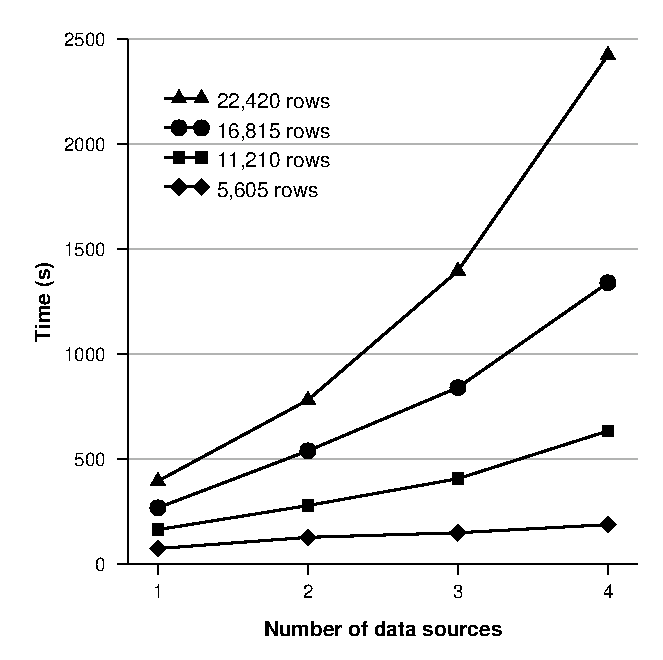
\includegraphics[width=\columnwidth,keepaspectratio]{run_times}}%
		\vskip 0.5cm%
	}}
	\caption{Execution time by data set and number of data sources (``push'' method)}
	\label{fig-run-times}
\end{figure}


At the other end of the scale, average execution times for the 22,420
row data set ranged from 395.6 seconds with one source up to 2,424.2
seconds (about 40 minutes) with four sources (see
Figure~\ref{fig-run-times}). In this instance the execution time with
four sources is over six times that with a single source, and appears to
be growing exponentially. Execution times for individual source machines
were again consistent, varying by no more than 1\% from the average.

These results were somewhat unexpected; while we had expected execution
times to increase with the number of source updates, we had not expected
them to increase quite so dramatically. Further investigation revealed
that some consumers progressed relatively normally, while others
appeared to progress in bursts. Since we were testing on an isolated
network, the most likely culprit is that multiple consumers were
blocking each other while attempting to simultaneously write to the
target. This problem could be solved by introducing an output queue
staging area between the consumers and the target, which would relieve
consumers of the need to deal with managing the target update process,
and present the target with an orderly sequence of updates, rather than
an overwhelming ``stampede''. It should be noted, however, that our
approach is designed primarily for ongoing update propagation, not
initial schema population. The volume of updates used in our testing
would seem unlikely for typical applications.

The results of comparing the Atom feed size with the consumer-generated
SQL code were also interesting. XML formats are generally very verbose,
so we expected the size of the Atom feeds to be greater than that of the
equivalent SQL commands. We were therefore surprised to find that the
opposite was the case, as shown in Figure~\ref{fig-sizes}. This was
sufficiently surprising that we at first suspected that we had
transposed the results! This was not the case, however.


\begin{figure}
	\fbox{\parbox[b]{.99\linewidth}{%
		\vskip 0.5cm%
		\centerline{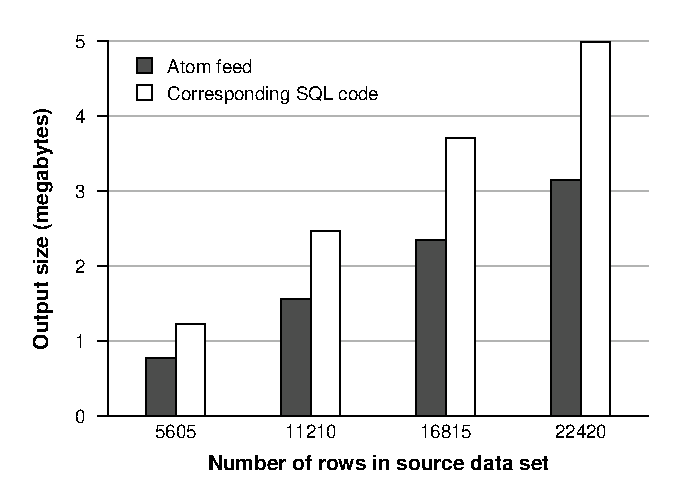
\includegraphics[width=\columnwidth,keepaspectratio]{output_sizes}}%
		\vskip 0.5cm%
	}}
	\caption{Comparison of Atom feed vs.\ SQL code size}
	\label{fig-sizes}
\end{figure}


As can be seen in Figure~\ref{fig-sizes}, the size of the generated SQL
code is generally about one and half times that of the corresponding
Atom feed. This bodes well for environments where bandwidth may be
limited. Compressing the feed would reduce the size further, something
that is not as readily achievable when sending SQL commands directly via
JDBC, for example.


\section{Future Work}
\label{sec-future-work}

As the initial prototype is intended as a basic proof of concept of our
approach, it has been kept as simple as possible in order to facilitate
implementation and testing. There are several obvious extensions to the
basic approach that will be investigated in later iterations.

First, we plan to repeat our tests after implementing the output queue
feature mentioned in Section~\ref{sec-results}, to see if this improves
matters (see Figure~\ref{fig-extended}). Later, we will implement a
transaction simulator to recreate a typical day-to-day production
environment and verify that the approach is effective under more typical
operating conditions. We will also compare our approach against existing
data integration solutions by means of a cost/benefit analysis, and may
investigate measuring various software quality characteristics as
defined by the ISO 9126 standard \cite{ISO-2001-9126-1}.


\begin{figure*}[htb]
	\fbox{\parbox[b]{.99\linewidth}{%
		\vskip 0.5cm%
		\centerline{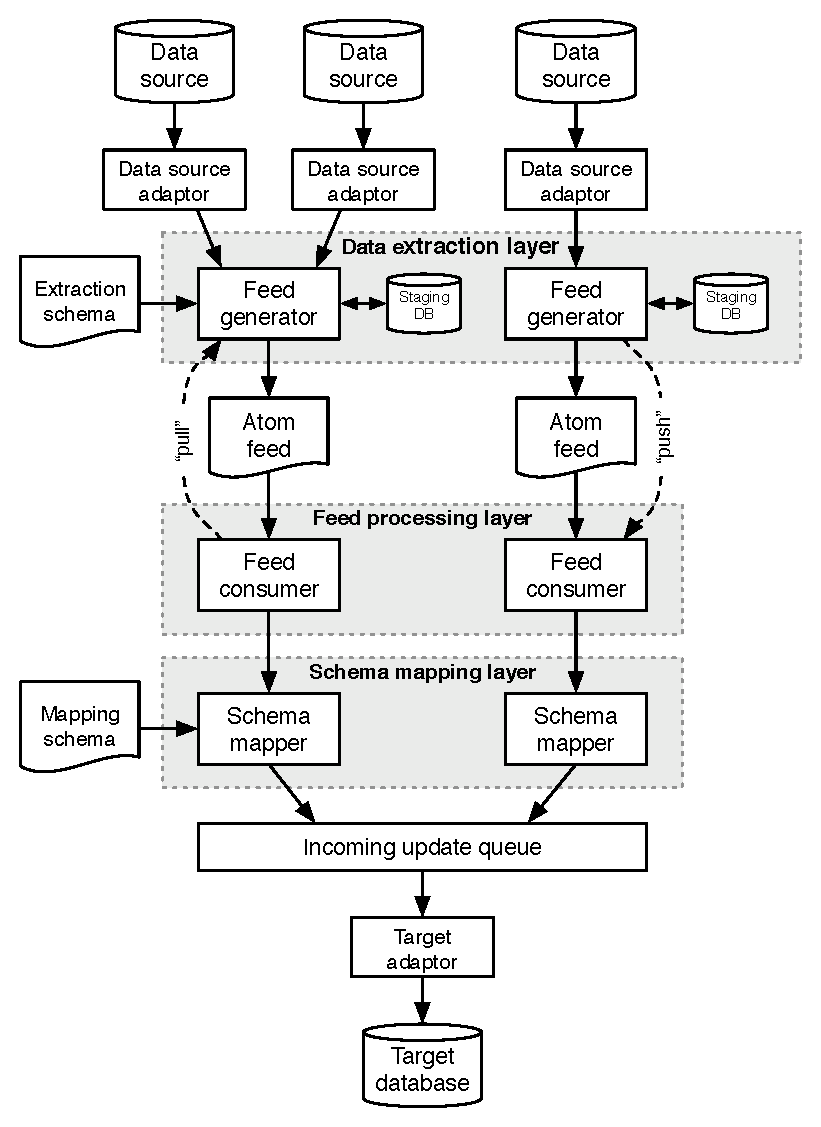
\includegraphics[scale=0.9]{Architecture_extended}}%
		\vskip 0.5cm%
	}}
	\caption{Possible extensions to the architecture}
	\label{fig-extended}
\end{figure*}


The prototype assumes that all data sources are homogeneous, that is,
that they all share the same semantics and schema. An obvious extension
is to permit heterogeneous data sources that have differing semantics
and schemas. This would require the addition of export and mapping
schemas, and a schema mapping layer to map incoming data from the source
schema to the target schema, as shown in Figure~\ref{fig-extended}.
These components could perhaps make use of the W3C's Web Ontology
Language (OWL) \cite{McGu-DL-2004-OWL} to specify mappings between
source and target schemas.

The prototype also assumes only a single data source underlying each
Atom feed (as implied by Figure~\ref{fig-basic}). It is quite feasible
to have a single feed that is effectively a view layered on top of a
collection of underlying databases, as illustrated at top left in
Figure~\ref{fig-extended} (e.g., a supplier might draw data for their
Atom feed from multiple databases within their organisation). It would
therefore be useful to investigate the possibility of multiple source
databases per Atom feed. Similarly, there is no particular reason to
restrict our approach to a single target database.

The prototype currently only supports the PostgreSQL and MySQL database
management systems (and has so far only been tested with MySQL). While
some simple generalisation has been done to enable the prototype to work
with with both products, an obvious extension is to further generalise
the data source interface to support multiple relational and
non-relational data sources and targets, as illustrated by the
``adaptor'' components in Figure~\ref{fig-extended}.

The data flows shown in Figures~\ref{fig-basic} and~\ref{fig-extended}
imply that our approach is one-way only (i.e., from the data sources to
the target database), but this may not be true in general. It would be
interesting to investigate the possibility of two-way data transfers,
i.e., allowing data to flow from the target back to the sources.

Another extension could be to generalise the ``transport layer'' of the
architecture. We currently use Atom feeds over HTTP connections, but
this may not be suitable for all applications. The architecture could be
generalised to support different transport formats such as UBL or binary
serialisations, and different transport protocols such as Jabber or
email, thus producing a fully-pluggable and very flexible architecture
that can be customised to suit any situation.

Other issues that could be investigated include transaction management,
concurrency control, how to deal with lost connections (rollback and
recovery), and so on.


\section{Conclusion}
\label{sec-conclusion}

In this paper, we discussed a lightweight approach for propagating
updates between databases, based on the Atom XML syndication format.
Cost is a major factor in the slow adoption of data integration
technologies by small to medium enterprises, so our approach could
provide a cost-effective alternative for implementing data integration
infrastructures in small business environments.

We have developed a basic proof of concept prototype that is being
evaluated using a series of realistic case studies. Preliminary results
suggest that our approach may not scale well with the number of data
source updates, but this may be due to congestion at the target and is
still under investigation. Somewhat unexpectedly, the preliminary
results also suggest that Atom provides a more compact representation
for propagating updates than sending SQL commands directly. This has
obvious potential for low bandwidth environments.

Our approach is very flexible and there are many interesting directions
in which it can be extended. We expect by the time of the conference to
have completed a more general implementation of the approach in Java,
and have more comprehensive results to report on.



\section*{Acknowledgements}
\label{sec-acknowledgements}

The authors would like to thank Dr.\ Colin Aldridge and Dr.\ Stephen
Cranefield for their helpful comments on an early draft of this paper.


\bibliographystyle{agsm}
\bibliography{Atom_updates}


\end{document}
